\section{Data Description}

\begin{figure*}[ht]
  \centering
  \subfigure[Number of records per user]{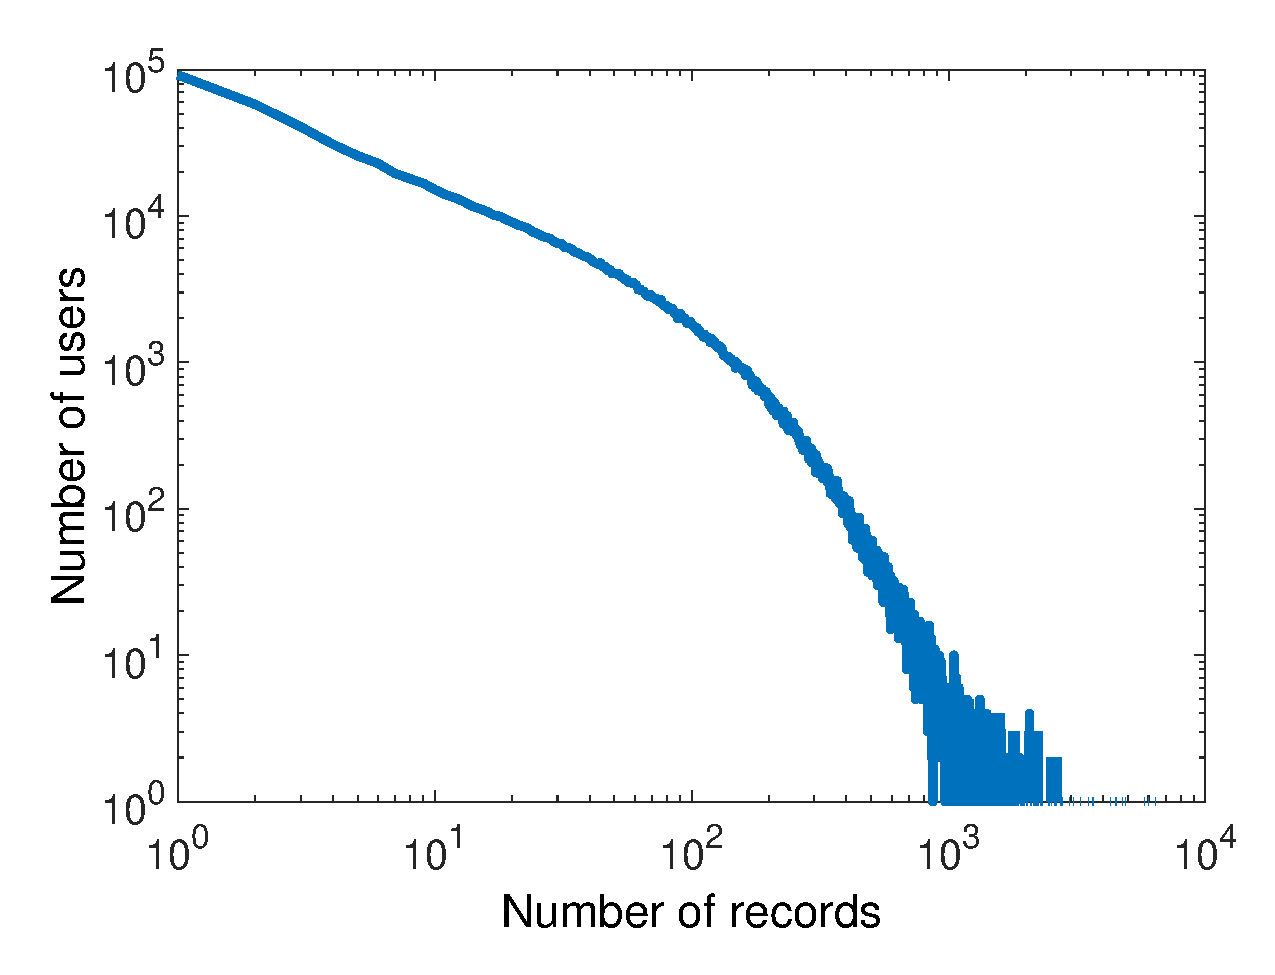
\includegraphics[width=0.32\textwidth]{figures/record_count_hist.pdf}}
  \subfigure[Time interval between consecutive records]{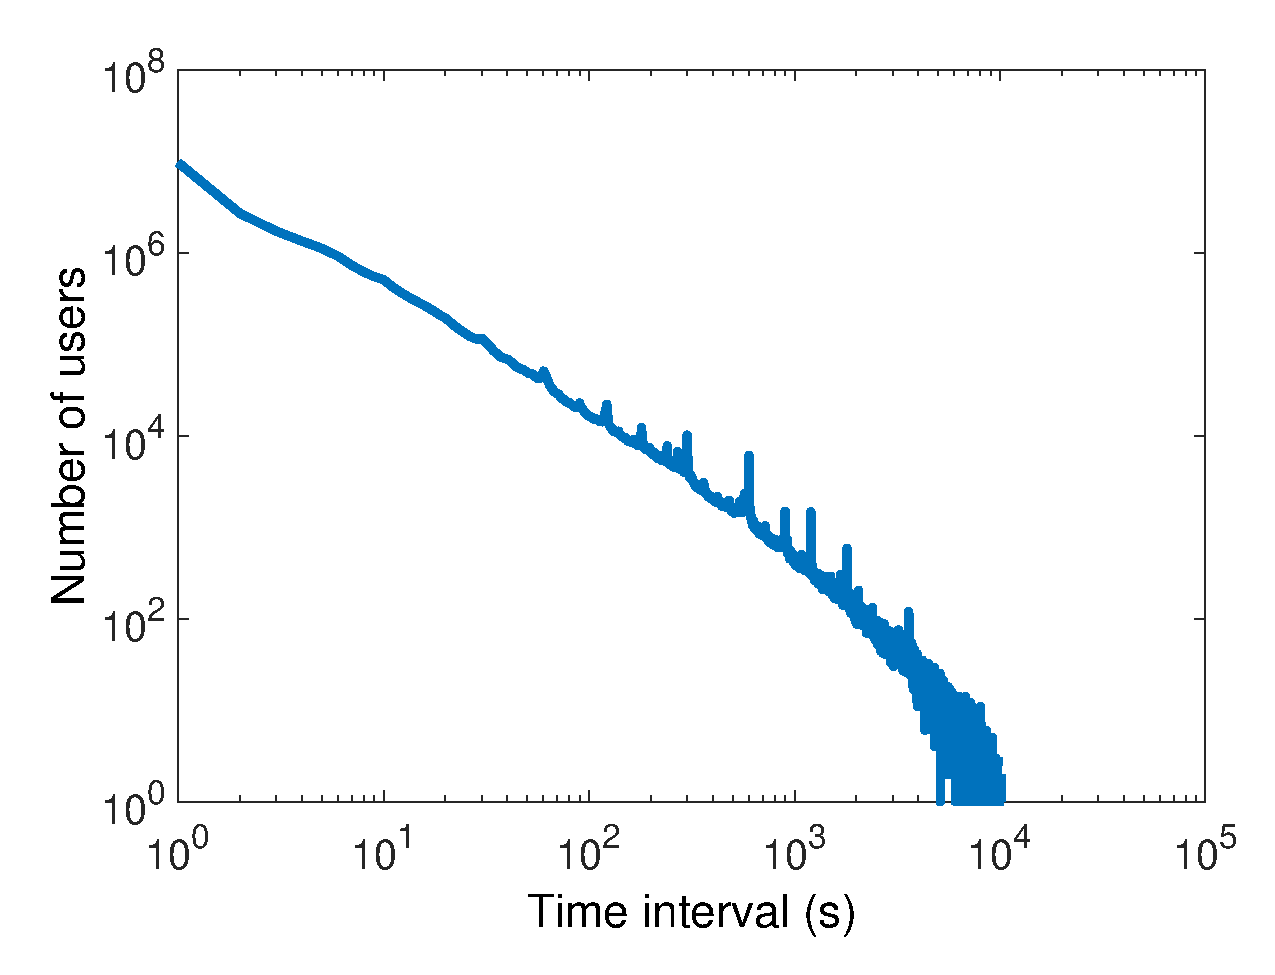
\includegraphics[width=0.32\textwidth]{figures/time_interval_hist.pdf}}
  \subfigure[Number of visited towers]{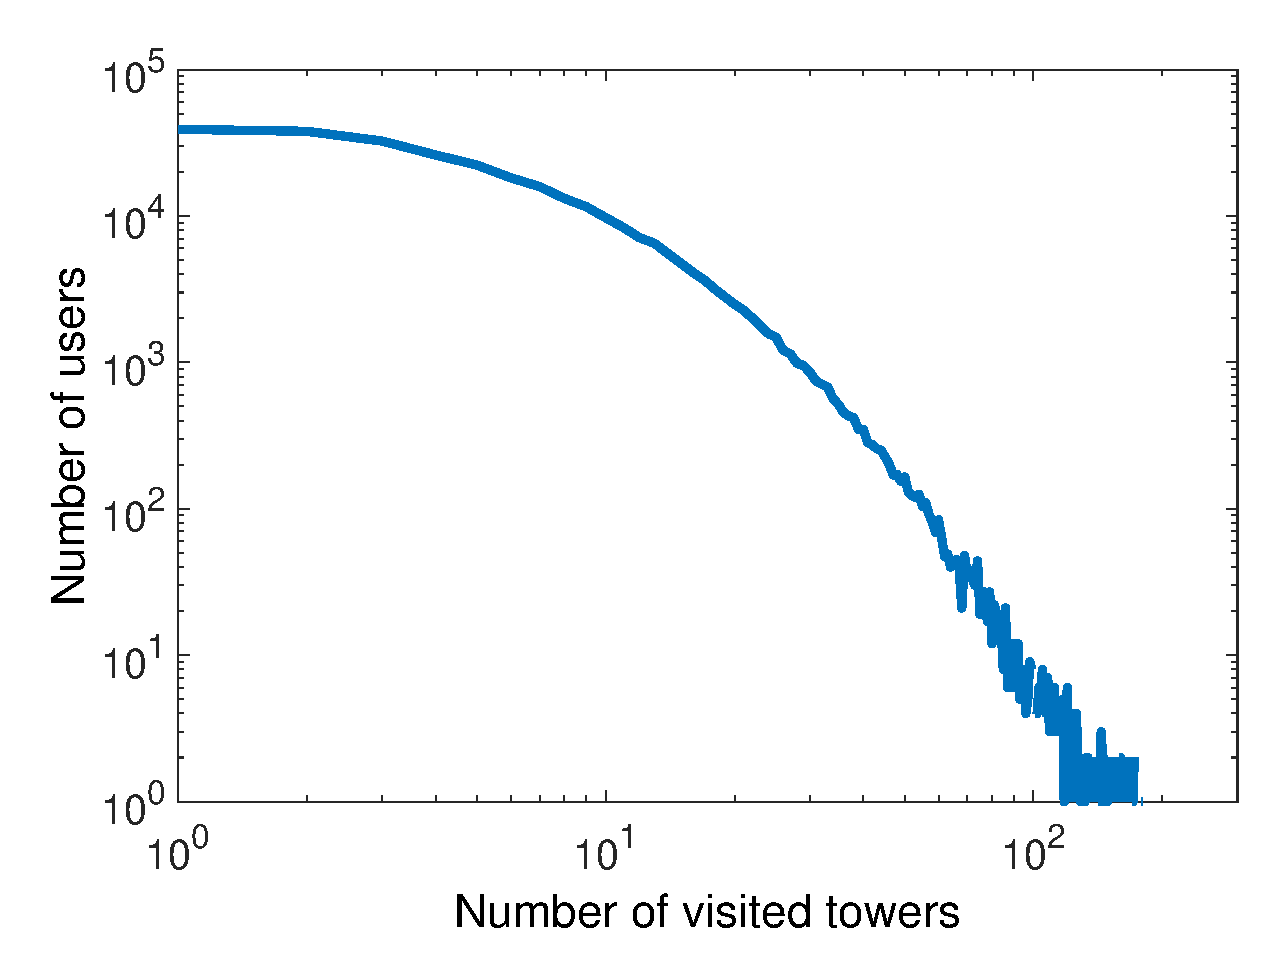
\includegraphics[width=0.32\textwidth]{figures/visited_tower_hist.pdf}}
  \caption{dataset statistics}
	\label{fig:data_stat}
\end{figure*}

Before we proceeding to the details of our approaches, we briefly introduce our dataset in this section. The dataset is mobile data access records provided by a cellular network operator in China. It was collected from three mid-size cities, including both urban and suburban area, during a three-hour period in the early evening (6pm - 9pm). The dataset includes more than 58 million mobile data access records with a total volume of more than 720 gigabytes, which covers all cell phones that were actively exchanging data with 5199 cell towers in the area during the observation period. The number of unique users included in this dataset is 0.9 million. And the total active time of all user is more than 1 million hours. 

Compared to similar data such as Call Detail Records (CDR), our dataset share same trends in several key statistics but is more dense temporally. For example, our dataset also have highly skewed distribution on number of records per user and time intervals between consecutive records as shown in Fig.~\ref{fig:data_stat}. Finer grained in temporal means better potential to infer user mobility even when the trip length is very short. Actually it is the case that most user only travelled a very short trip in terms of number of visited towers according to Fig.~\ref{fig:data_stat}.

\subsection{An example user's trace}

\begin{figure}[h]
    \centering
    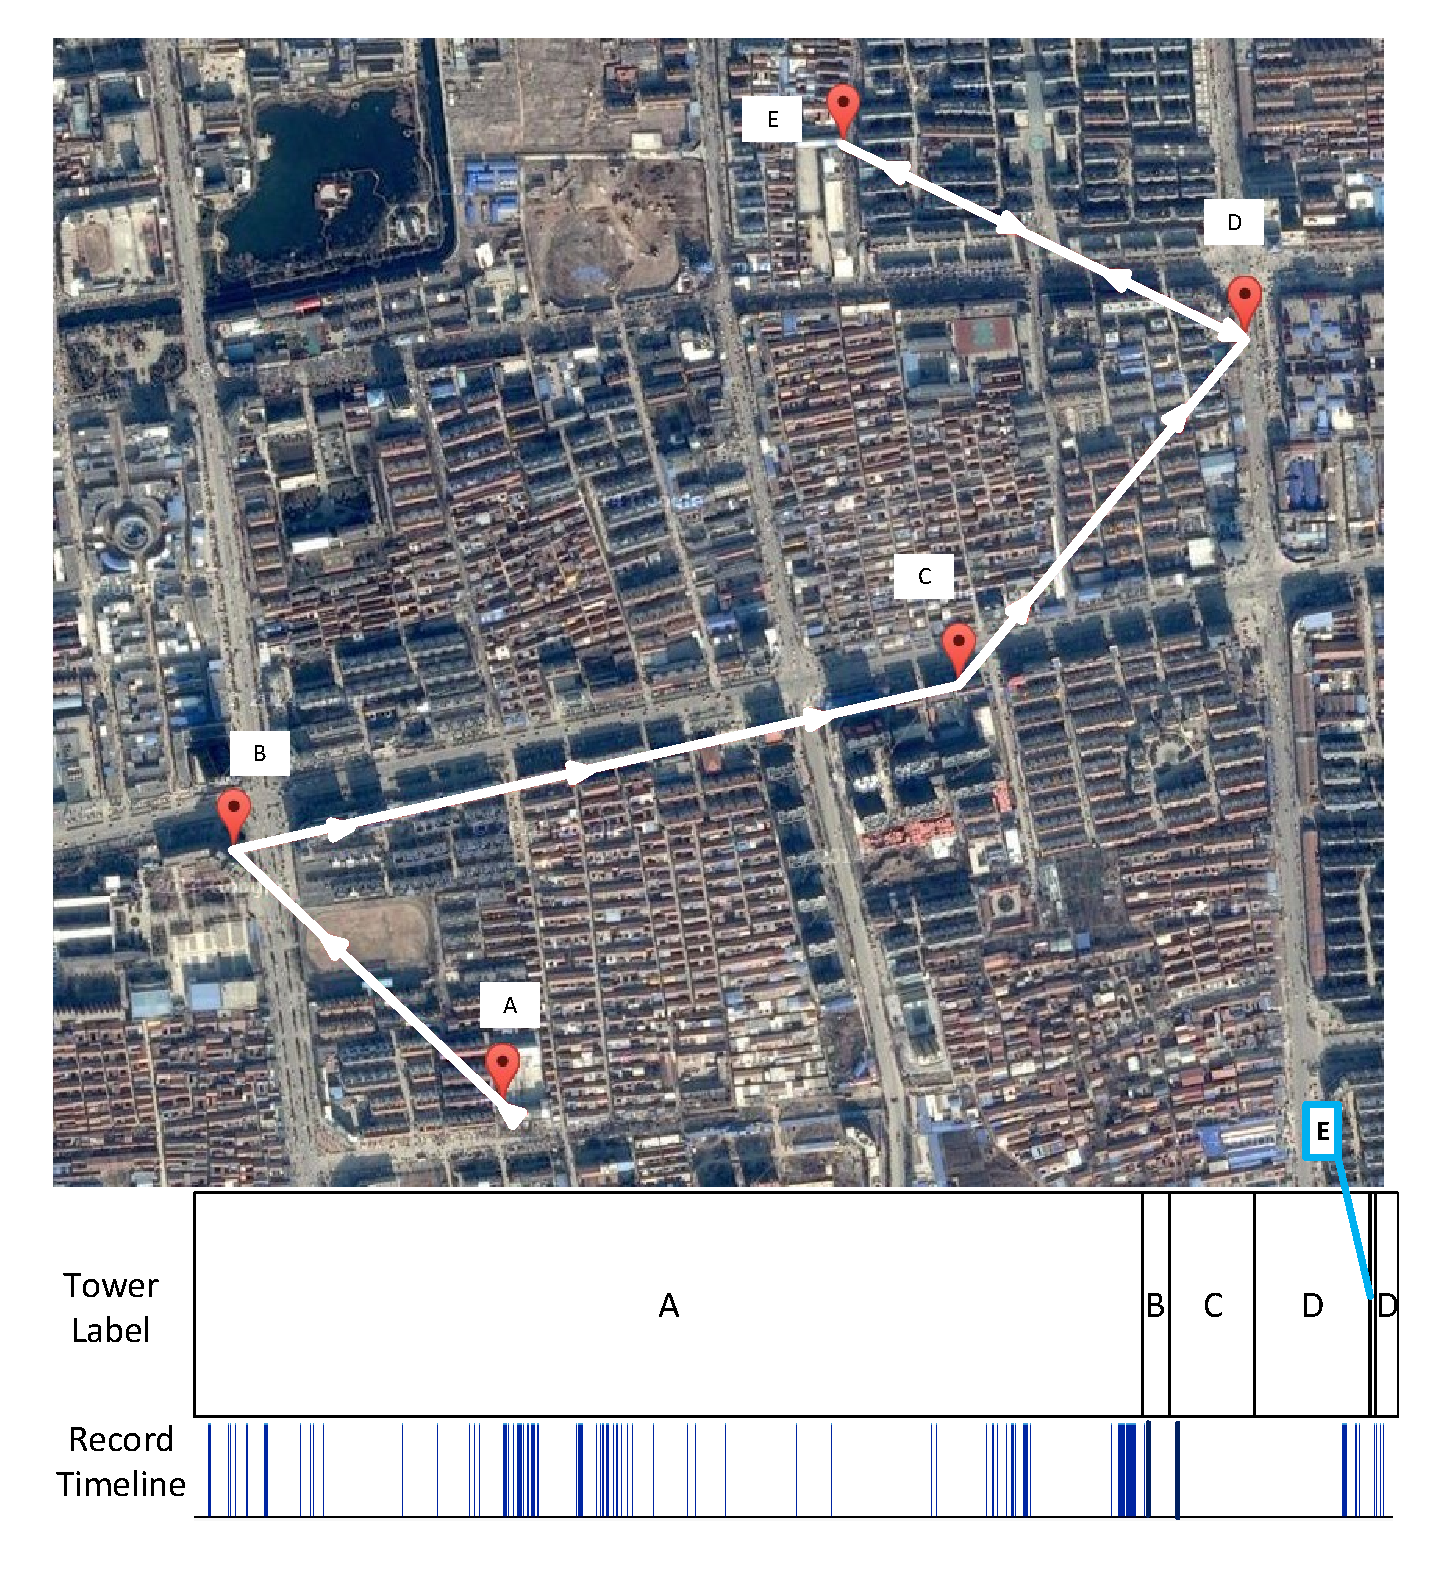
\includegraphics[width=\linewidth]{./figures/typical_user.pdf}
    \caption{A typical data access session of a user.}
    \label{fig:typical_user}
\end{figure}

To show a clear view of our trace and serve as a running example, we have selected a random user from the dataset and show his mobile data access trace in fig.~\ref{fig:typical_user}. The figure contains two parts. The top part is a map shown the towers that were visited by the user. We use markers to show tower locations and arrowed lines to show the sequence of visiting. The bottom part of the figure shows the time line of the user's data access records with pulses, each pulse represent a mobile data access record and its position on the time line shows its relative time. We also show to which tower the user is communicated for each mobile data access with tower labels above the pulses. So for this particular user, he communicate with tower A for a quite long time, and shortly connected to tower B then swithed to tower C. After a while, the user was found in tower D's coverage area. After a while, he connected to tower E for a very short time, and then switch back to tower D.